% *******************************************************************************
% * Copyright (c) 2007 by Elexis
% * All rights reserved. This document and the accompanying materials
% * are made available under the terms of the Eclipse Public License v1.0
% * which accompanies this distribution, and is available at
% * http://www.eclipse.org/legal/epl-v10.html
% *
% *  $Id: varianten.tex 2469 2007-06-02 19:47:42Z rgw_ch $
%
%*******************************************************************************
% !Mode:: "TeX:UTF-8" (encoding info for WinEdt)

\section{Das Programm allein in verschiedenen Varianten}
\label{varianten}
Am Anfang dieses Buchs (s. S. \pageref{easyinstall}) sahen Sie die einfache Standardinstallation. Wenn Sie mehr Kontrolle über die heruntergeladenen Dateien und die Art der Konfiguration möchten, können Sie auch einzelne Bestandteile des Programms beziehen. Die Erläuterung, was Sie benötigen, finden Sie in den
weiteren Abschnitten dieser Seite.

Es muss aber darauf hingewiesen werden, dass alle unten aufgeführten Downloads eine leere Datenbank anlegen, welche erst nach einer nicht ganz trivialen
Grundkonfiguration benutzbar ist. Wir empfehlen zum Ausprobieren lieber die 
Standardinstallation.

\section{Verschiedene Installer-Typen}
Elexis baut auf einer sogenannten \textit{Eclipse Rich Client} Umgebung auf, diese wiederum auf
einem \textit{Java Runtime Environment}, und dieses wiederum auf dem Betriebssystem Ihres Computers. Auch OpenOffice ist im Betriebssystem eingebettet und kooperiert sowohl mit der Java Runtime als auch mit dem Betriebssystem und Elexis direkt. Folgende Grafik soll diese Zusammenhänge verdeutlichen:
\begin{figure}[hb]
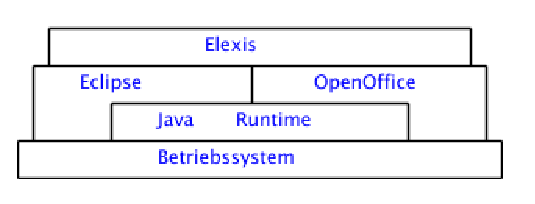
\includegraphics{images/modell}
\caption{Elexis Modell}
\label{Aufbau von Elexis}
\end{figure}

Je nachdem, was schon auf dem Zielcomputer installiert ist, braucht man also ein mehr oder weniger umfangreiches Paket.

\section{Komplettpaket inklusive JRE}

Dies benötigen Sie, wenn Sie noch keine Java-Runtime auf Ihrem System haben, und wenn Sie Elexis das erste Mal installieren. Sie können folgendermassen prüfen, ob Sie eine Java-Runtime installiert haben:

Öffnen Sie eine Kommandozeile (in Windows: cmd.exe, bei Mac und Linux: Terminal bzw. xterm) tippen Sie ein:

\textit{java -version} \texttt{Eingabetaste}

Wenn jetzt eine Fehlermeldung kommt (Befehl oder Datei nicht gefunden), dann haben Sie Java nicht oder nicht korrekt installiert. Wenn eine Version kleiner als 1.5 kommt, dann haben Sie eine zu alte Version. In diesen Fällen brauchen Sie dieses Paket:
\begin{itemize}
 \item Kompletter Installer für Windows:  \href{http://www.elexis.ch/download.php?file=demo} {elexis-win32-jre.exe}
\item Kompletter Installer für Linux x86:  \href{http://www.elexis.ch/download.php?file=elexis-linux-jre-i386}{elexis-linux.i386-jre.run}


\end{itemize}


Anmerkung
Die Installation wird (ausser dem Platzverbrauch von ca. 50MB) keine Veränderung an Ihrem Computer bewirken. Auch die Java Runtime wird nur lokal innerhalb des Elexis-Verzeichnisses erstellt und kann mit diesem leicht wieder entfernt werden.
%
%hier fehlen noch die url
%
\subsection{Komplettpaket ohne JRE}
Dies benötigen Sie, wenn Sie eine Java Runtime, aber bisher noch nie Elexis auf Ihrem System installiert haben
\begin{itemize}
 \item Installer für Windows:  \href{http://www.rgw.ch/download.php?file=elexis-win32}{elexis-win32.exe}
\item Installer für Linux x86:  \href{http://www.elexis.ch/download.php?file=elexis-linux-i386}{elexis-linux-i386.run}
\item Archiv für MacOS X (10.4 oder höher): \href{http://www.elexis.ch/download.php?file=elexis-mac}{Installer, ca. 25MB}
\end{itemize}

\subsection{Plugin allein}
Dies benötigen Sie, wenn Sie Elexis schonmal installiert haben, und nur eine neuere Version installieren möchten. Das Plugin ist für alle Betriebssysteme dasselbe, es gibt deshalb nur eine Datei.
\begin{itemize}
 \item Alle Systeme:  \href{http://www.elexis.ch/download.php?file=elexis-plugin}{elexis-plugin.zip, ca. 5MB}
\item \href{http://www.elexis.ch/download.php?file=demodaten.zip}{Demo-Datenbank, ca. 12MB}
\end{itemize}

\subsection{Demo-Datenbank}
Wenn Sie Elexis ohne Konfiguration ausprobieren möchten, laden Sie die
Demo-Datenbank herunter (ca. 11 MB). Entpacken Sie diese Zipdatei in Ihrem Elexis-Ord\-ner
(So dass im Elexis-Ordner dann die Unterordner \textit{Plugins}, \textit{Con\-figu\-ra\-tion}, ev. \textit{work\-space}
und neu \textit{demoDB} zu finden sind, nebst den Dateien Elexis.exe, Elexis.ini und anderen.

Elexis greift, wenn es beim Start einen demoDB-Ordner in seinem Verzeichnis vorfindet, nur noch auf diese
 Datenbank zu, egal was sonst eingestellt wurde. Wenn Sie also wieder auf eine andere Datenbank zugreifen wollen,
 müssen Sie den Ordner \textit{demDB} löschen oder umbenennen.

Um sich in der demoDB als Anwender einzuloggen, geben Sie als Name und Passwort jeweils \textit{test} ein (ohne die Anführungszeichen), der Administrator-Account hat den Namen Administrator und das Passwort admin.
\section{Downloads}
Hier finden Sie verschiedene Varianten der Datei. %Genauere Erklärungen zur Bedeutung der einzelnen Files finden Sie auf der Seite ellen}.
\subsection{Druckbare  Anleitungen zum Einstieg}

\begin{itemize}
 \item \href{http://www.elexis.ch/files/erste_schritte.pdf}{Installationsanleitung und Kurzhandbuch erste Schritte (PDF)}
\item \href{http://www.elexis.ch/files/pat_agenda.pdf}{Einführung Patient erfassen und Agenda einrichten}
\end{itemize}

\subsection{Programm für Microsoft Windows (2000, XP Home oder XP pro)}
\begin{itemize}
\item \href{http://www.elexis.ch/download.php?file=demo}{Komplett mit OpenOffice, Java und Beispieldaten (ca. 150 MB)}
\item \href{http://www.rgw.ch/download.php?file=elexis-jre-win32}{Installer mit Java runtime (ca. 40MB)}
\item \href{http://www.rgw.ch/download.php?file=elexis-win32}{Installer ohne Java runtime ca. 20MB)}
\end{itemize}

\subsection{Programm für Linux i386 (oder AMD64)}
\begin{itemize}
 \item \href{http://www.elexis.ch/download.php?file=elexis-linux-jre-i386}{Installer mit Java runtime (ca. 50 MB)}
\item \href{http://www.elexis.ch/download.php?file=elexis-linux-i386}{Installer ohne Java runtime (ca. 30 MB)}
\end{itemize}

\subsection{Programm für Apple Macintosh ab OSX 10.4 (Tiger)}
\begin{itemize}
 \item \href{http://www.elexis.ch/download.php?file=elexis-mac}{Installer (ca. 25MB)}
\end{itemize}

\subsection{Alle Systeme:}
\begin{itemize}
 \item \href{http://www.elexis.ch/download.php?file=elexis-plugin}{Elexis-Plugin allein (ca. 5MB)}
\item \href{http://www.elexis.ch/download.php?file=demodaten.zip}{Demo-Datenbank  (ca. 12MB) }
\end{itemize}

\subsection{Stammdaten:}
\begin{itemize}
 \item \href{http://cug.zur-rose.ch/aerztegrossist/aerztegrossist.asp}{Medikamentenstamm. (Kostenlos nur für Kunden der Apotheke zur Rose,  ASAS-Login)}
\item \href{http://www.polymed.ch/d/aktuell/downloads.html}{Polymed-Artikelstamm}
\item \href{http://www.tarmedsuisse.ch/fileadmin/media/Dateien/Browser/TARMED_Database_1.03.zip}{Tarmed-Datenbank}
\item \href{http://www.dimdi.de/dynamic/de/klassi/downloadcenter/icd-10-gm/version2006/systematik/x1gea2006.zip}{ICD-10}
\item \href{http://www.famh.ch/liste_analyses_d_06.pdf}{Analysenliste (nur PDF erhältlich)}
\item \href{http://www.bag.admin.ch/themen/krankenversicherung/02874/index.html?lang=de&download=M3wBUQCu/8ulmKDu36WenojQ1NTTjaXZnqWfVpzLhmfhnapmmc7Zi6rZnqCkkIV6e3l9bKbXrZ2lhtTN34al3p6YrY7P1oah162apo3X1cjYh2+hoJVn6w==}{MiGeL (nur PDF)}
\end{itemize}

